\documentclass[10pt,a4paper]{article}
\usepackage[utf8]{inputenc}
\usepackage{amsmath}
\usepackage{amsfonts}
\usepackage{amssymb}
\usepackage{pgfplots}
\author{az}
\title{Notes on ML Study}
\date{\today}
\begin{document}
\maketitle
\tableofcontents
\newpage



\section{Above All}

\paragraph{
I' like to write down the long walking that I will have to go pass on the way to learn ML.
}


\section{Logs}


\subsection{10.24}
\subsubsection{ML Formula}
\paragraph{Least Squared Method}

$$
\begin{cases}
LS
& \boldsymbol{\theta}^* =\boldsymbol{\Phi}^\dagger\boldsymbol{y}
\\
LA
&\widehat{\boldsymbol{\theta}} = (\boldsymbol\Phi^\top \widetilde{W}\boldsymbol{\Phi})^\dagger\boldsymbol\Phi^\top \widetilde{W}\boldsymbol{y}
\\
Hugger
& \widehat{\boldsymbol{\theta}} = (\boldsymbol\Phi^\top \widetilde{W}\boldsymbol{\Phi}+ \lambda\boldsymbol\Theta^\dagger)^\dagger\boldsymbol\Phi^\top \widetilde{W}\boldsymbol{y}
\\
Tukey
& TBD
\\
0/1
& TBD
\\
Ramp
& \widehat{\boldsymbol{\theta}} = (\boldsymbol\Phi^\top {W}\boldsymbol{\Phi}+ \lambda\boldsymbol I)^\dagger\boldsymbol\Phi^\top {WV}\boldsymbol{y}
\end{cases}
$$

$$
\begin{cases} 
LS  	&\|\Delta\|_2   
\\

LA 	&\|\Delta\|_1
\\

Hugger & \sum\rho_{Huger}(r), 
    \rho_H = \begin{cases}
    r^2/2 &(|r| \le \eta)\\
    \eta|r|-\eta^2/2  (|r| > \eta)
    \end{cases}
\\

Tukey  & \sum\rho_{Tukey}(r),
    \rho_T =  \begin{cases}
        \frac{\left(1- [1-\frac{r^2}{\eta^2}]^3 \right)\eta^2}{6},
        &|r|\le\eta
        \\
        
        \frac{\eta^2}{6}, &|r| > \eta
    \end{cases}
\\

0/1 
	& \frac{1}{2}\sum_{i=1}^n \left(sign(\hat{y}_i)-y_i\right)^2
	 sign(m) = \begin{cases}
		 +1 & m > 0 \\
		 0  & m = 0  \\
		 -1 & m < 0
	\end{cases}	
\\

0/1 
	&\frac{1}{2}\sum_{i=1}^n\left( 1 - sign(\hat{y}_i)y_i \right)
\\
Ramp
    & \sum_{i=1}^n \gamma(1-\hat{y}_iy_i)
     \gamma(m)=\min \left\{ 1, \max(0,1-m) \right\}= 	           
    \begin{cases}
        1          &(m < 0) \\
        1-m       &(0\le m \le 1) \\
        0          &(m > 1)
    \end{cases}

\end{cases}
$$


\subsubsection{Tips for latex}
\paragraph{
Latex is a really powerful tool. I start to use it to write article and notes. 
} 
\subparagraph{Question for it:}
\begin{itemize} %enumerate
 \item align
 \item list
 \item tables
\end{itemize}
%
%
\pgfplotsset{width=6cm,compat=1.9}
\subsection{10.25}
\paragraph{Start to learn plotting pictures}
\subparagraph{Ref: https://blog.csdn.net/stereohomology/article/details/24266409}
\begin{tikzpicture}
\begin{axis}
\addplot[color=red]{exp(x)};
%\addplot[color=blue]{ln(x)};
\addplot[color=green]{x^2};
\end{axis}
\end{tikzpicture}
%Here ends the furst plot
\hskip 5pt
%Here begins the 3d plot
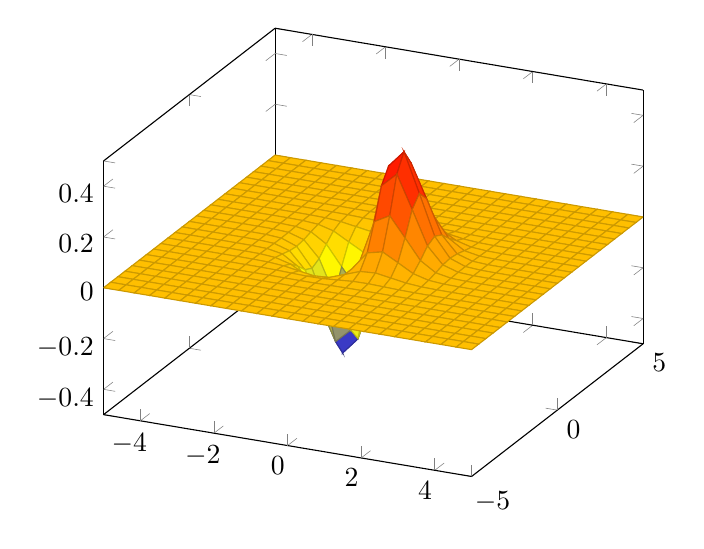
\begin{tikzpicture}
\begin{axis}
\addplot3[
    surf,
]
{exp(-x^2-y^2)*x};
\end{axis}
\end{tikzpicture}



\end{document}